%==============================================================================
\section{Multi-Antenna Receivers, Latency and Robustness}
\label{sec:regime}
%==============================================================================

\subsection{Common Receive Combiner}

With $M>1$ antennas the FC must choose one combiner $\vm$ for all devices without knowing the weights. Maximizing $\min_j|\vm^{\mathsf H}\vh_j|^2$ protects the weakest link regardless of where the mass lies. We use a reweighted principal-eigenvector heuristic for this max--min problem and the least-squares equal-gain combiner, and keep the better of the two per instance. The gains $g_j$ are then dependent and Theorem~\ref{thm:bottleneck} no longer holds exactly, but it still brackets the bottleneck.

\begin{proposition}[Combiner bounds]\label{prop:combiner}
Let $\vh_j\sim\mathcal{CN}(\mathbf{0},\beta_j\mathbf{I}_M)$ be independent and let $B_{\vm}=\max_jd_j^2/|\vm^{\mathsf H}\vh_j|^2$ for a unit-norm combiner $\vm$ that may depend on the channels. For every $x>0$,
\begin{equation}
\Prob\{B_{\vm}\le x\}\le\prod_{j=1}^NQ\Big(M,\frac{d_j^2}{\beta_jx}\Big),
\label{eq:comb_upper}
\end{equation}
i.e., $B_{\vm}$ is stochastically larger than the bottleneck of device-side maximum-ratio transmission, whose law is~\eqref{eq:bottleneck_m} with $m=M$ and mean gains $M\beta_j$. If $\vm$ maximizes $\min_j|\vm^{\mathsf H}\vh_j|^2$, then also
\begin{equation}
\Prob\{B_{\vm}\le x\}\ge\exp\Big(-\frac{d_{\max}^2}{x}\sum_{j=1}^N\frac{1}{\beta_j}\Big),\qquad d_{\max}=\max_jd_j.
\label{eq:comb_lower}
\end{equation}
\end{proposition}

To see how much a common combiner loses, we optimized the combiner numerically (SLSQP with five starts) on Rayleigh channels with attention weights of Qwen3-4B at 8k context, for $M=4,8$ and $N=8$--$64$. Optimizing the max--min objective raises the minimum gain by a median of 5.1--11.0~dB over the heuristic, but it improves the bottleneck $B$ by only 0.4--1.8~dB and worsens it in 36--45\% of the instances, because lifting the weakest link lowers the gains of the devices that hold the mass. The optimized combiners remain a median of 4.3--9.6~dB above the bound~\eqref{eq:comb_upper}: without the weights, a common combiner recovers little of the per-device diversity.

When $M\ge N$, zero-forcing (ZF) separates the devices in one slot, and the FC can recover every $\obar_j$ and compute the ratio with digitally reported weights~\cite{chen2024view}. Over-the-air aggregation is therefore of interest for $N>M$, where the orthogonal alternative is ZF in $\lceil N/G\rceil$ slots of $G\le M$ devices each; we use $G=\max(1,M/2)$, for which the mean ZF noise enhancement is finite.

\subsection{Latency at Matched Accuracy}

Per layer and decoded token, every scheme starts with the query broadcast. Let $\tau$ be the duration of one downlink--uplink exchange, $R$ the uplink RE rate and $\rho$ the spectral efficiency of the digital uplink, which multiplexes $\mu=\min(M,N)$ devices; the analog streams are packed in phase and quadrature, two per RE. An analog scheme whose required SNR exceeds the operating SNR repeats its payload $r=\lceil10^{(\snr_{\rm req}-\snr)/10}\rceil$ times. With $T_{\rm a}=rH(d_v+1)/(2R)$ for the analog payload and $T_{\rm d}(n)=n/(\rho\mu R)$ for $n$ digital bits, the per-layer latencies of the proposed design are
\begin{align}
T_{\rm tone}&=2\tau+\frac{HL\nu}{R}+\max\{T_{\rm a},T_{\rm d}(NHb_A)\},\\
T_{\rm dig}&=2\tau+T_{\rm d}(NHL\log_2q)+\max\{T_{\rm a},T_{\rm d}(NHb_A)\},
\end{align}
where $b_A$ is the ring size of the secure sum of the arrived weights. Known-weight aggregation takes $2\tau+T_{\rm d}(NHb_w)+T_{\rm a}$ with $b_w$-bit weights, time-division ZF $\tau+\max\{r\lceil N/G\rceil Hd_v/(2R),T_{\rm d}(NHb_w)\}$, and a digital merge of all partials with $b$-bit values
\begin{equation}
T_{\rm merge}(b)=\tau+T_{\rm d}\big(NH(d_v+1)b\big).
\label{eq:Tmerge}
\end{equation}
The relevant competitor for privacy is a \emph{secure digital merge}, which securely aggregates all $NH(d_v+1)$ partials and therefore reveals only the sums. Secure aggregation adds masks but no payload, so its latency is~\eqref{eq:Tmerge}; what matters is the ring size $b$ at which the fixed-point sums are accurate enough. With an offline scale per head, it must cover the dynamic range of the partials across queries; a per-instance scale needs fewer bits but a handshake of its own, i.e., a second round trip. We measure both ring sizes at the accuracy target of Section~\ref{sec:exp} rather than assume them. The analog designs pay off for many devices or narrow bands, and the extra round trip of the handshake is their main cost. Fig.~\ref{fig:regime} shows the fastest scheme in the $(N,\text{bandwidth})$ plane.

\begin{figure}[t]
\centering
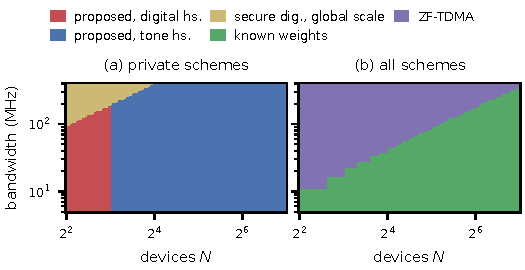
\includegraphics[width=\linewidth]{fig_regime.pdf}
\caption{Fastest scheme per token in the $(N,\text{bandwidth})$ plane, Qwen3-4B, $M=4$, $\tau=0.5$~ms, operating SNR 15~dB, with the required SNRs of the 8k sweep, $L=32$, $\nu=4$ and the measured ring sizes of Section~\ref{sec:exp}: (a) among schemes that reveal neither weights nor per-device data; (b) among all schemes.}
\label{fig:regime}
\end{figure}

\subsection{Robustness}

\emph{Common-mode errors.} A gain error common to all streams of all devices cancels in the analog ratio~\eqref{eq:estimator}; in the split ratios it scales the numerator only, so the FC must calibrate its own gain.

\emph{Device-specific errors.} Imperfect CSI or a residual phase at device $j$ multiplies its streams by a complex factor whose real part $\lambda_j$ attenuates them and whose imaginary part leaks each stream into its quadrature partner. Unlike saturation, the device does not know $\lambda_j$, so the arrived weight is $\lambda_ja_j$ while it reports $a_j$: by Proposition~\ref{prop:selfconsistency} the numerator shrinks by $\sum_j(1-\lambda_j)a_j\obar_j$. For a phase error of standard deviation $\sigma_\phi$ this is a common shrinkage of about $\sigma_\phi^2/2$, i.e., 1.5\% at $10^\circ$ and 6\% at $20^\circ$.

\emph{Frequency selectivity.} By Corollary~\ref{cor:coherence}, a payload that spans $C$ coherence blocks costs a non-saturating design $10\log_{10}C$~dB when the devices back off to their weakest block.

\emph{Heterogeneous path loss.} By Theorem~\ref{thm:bottleneck}, large-scale gains enter through $S=\sum_jd_j^2/\beta_j$: a device that holds mass behind a weak link dominates the bottleneck of a non-saturating design. The noise-matched report caps such a device automatically (Proposition~\ref{prop:kappa}) but attenuates its data. A digital fallback avoids this loss: the $k\ge2$ devices with the weakest effective gains, which the FC selects from the gains alone, securely aggregate their partials $(d_j,\vn_j)$ instead of transmitting over the air, and the FC adds their exact sum to its anchor. The cost is $kH(d_v+1)$ masked values per layer.
